\documentclass[a4j,11pt,twoside]{ujbook}
\usepackage{ascmac}
\usepackage[dvipdfmx]{graphicx}
\usepackage{matx}
\usepackage{manyfloat}
\begin{document}
%--------------------------------------------
% タイトルページ
\title{倒立振子の安定化制御}
\author{瀧川文哉}
\date{2017年7月}
\maketitle
%--------------------------------------------
% 目次
\pagenumbering{roman}
\tableofcontents
\listoffigures
\listoftables
\cleardoublepage
\pagenumbering{arabic}
%--------------------------------------------
% 本文
\chapter{はじめに}
\section{実験目的}
本実験の目的は倒立振子の安定化制御の制御系の設計を状態空間法を用いて行うことにより、線形時不変システムに対する設計法を習得することである。
\section{制御対象と制御目的}
\subsection{倒立振子系}
制御対象として、図\ref{fig:倒立振子系}に示されるような倒立振子系を考える。モノレール上に台車が置かれ、台車上のモノレールと直角な軸に一本の棒が取り付けられ、棒はその軸まわりに自由に回転できる。台車はベルトとプーリを介して、モータにより駆動され、モノレール上を走行できる。すなわち、棒(振子)は鉛直線とモノレールにより定まる平面に拘束されて、台車によって動かされるようになっている。

\subsection{観測出力と操作入力}
倒立振子系の観測出力として、ポテンショメータにより、次の2つが測定できる。
\begin{description}
	\setlength{\itemindent}{0pt}
	\item[1°] 台車の基準位置からの変位$r$に比例する電圧$y_1$
	\item[2°] 棒の鉛直線となす角度$\theta$に比例する電圧$y_2$
\end{description}
一方、操作入力は、つぎのものである。
\begin{description}
	\setlength{\itemindent}{0pt}
	\item[1°] モータの駆動アンプへの入力電圧$u$
\end{description}
ここで、モータにより駆動される台車には、$u$に比例した駆動力が働くものとする。
\subsection{制御目的}
この倒立振子系は、2つの平衡点をもつ。1つは棒が鉛直線に沿って垂れ下がった状態、もう一つは棒が鉛直線に沿って倒立した状態である。前者は、棒を揺らせば、いわゆる振子となり、揺らせれば、いわゆる振子となり、ゆれは時間が立てば止まるので、安定平衡点である。後者は、いわゆる倒立振子であるが、倒立状態にある棒を少しでもつつけば、真っ逆さまに落ちていくので、不安定平衡点である。このような倒立振子系に対する制御目的として、つぎを考える。
\begin{description}
	\setlength{\itemindent}{0pt}
	\item[1゜]倒立状態にある棒が何らかの原因で傾いたとき、台車を動かして、棒をすみやかに倒立状態に戻す(不安定抵抗店の安定化)。
	\item[2゜]倒立位置を指定した位置に移動させる。
\end{description}
% 1.1図の挿入
\begin{figure}[htbp]
	\begin{center}
		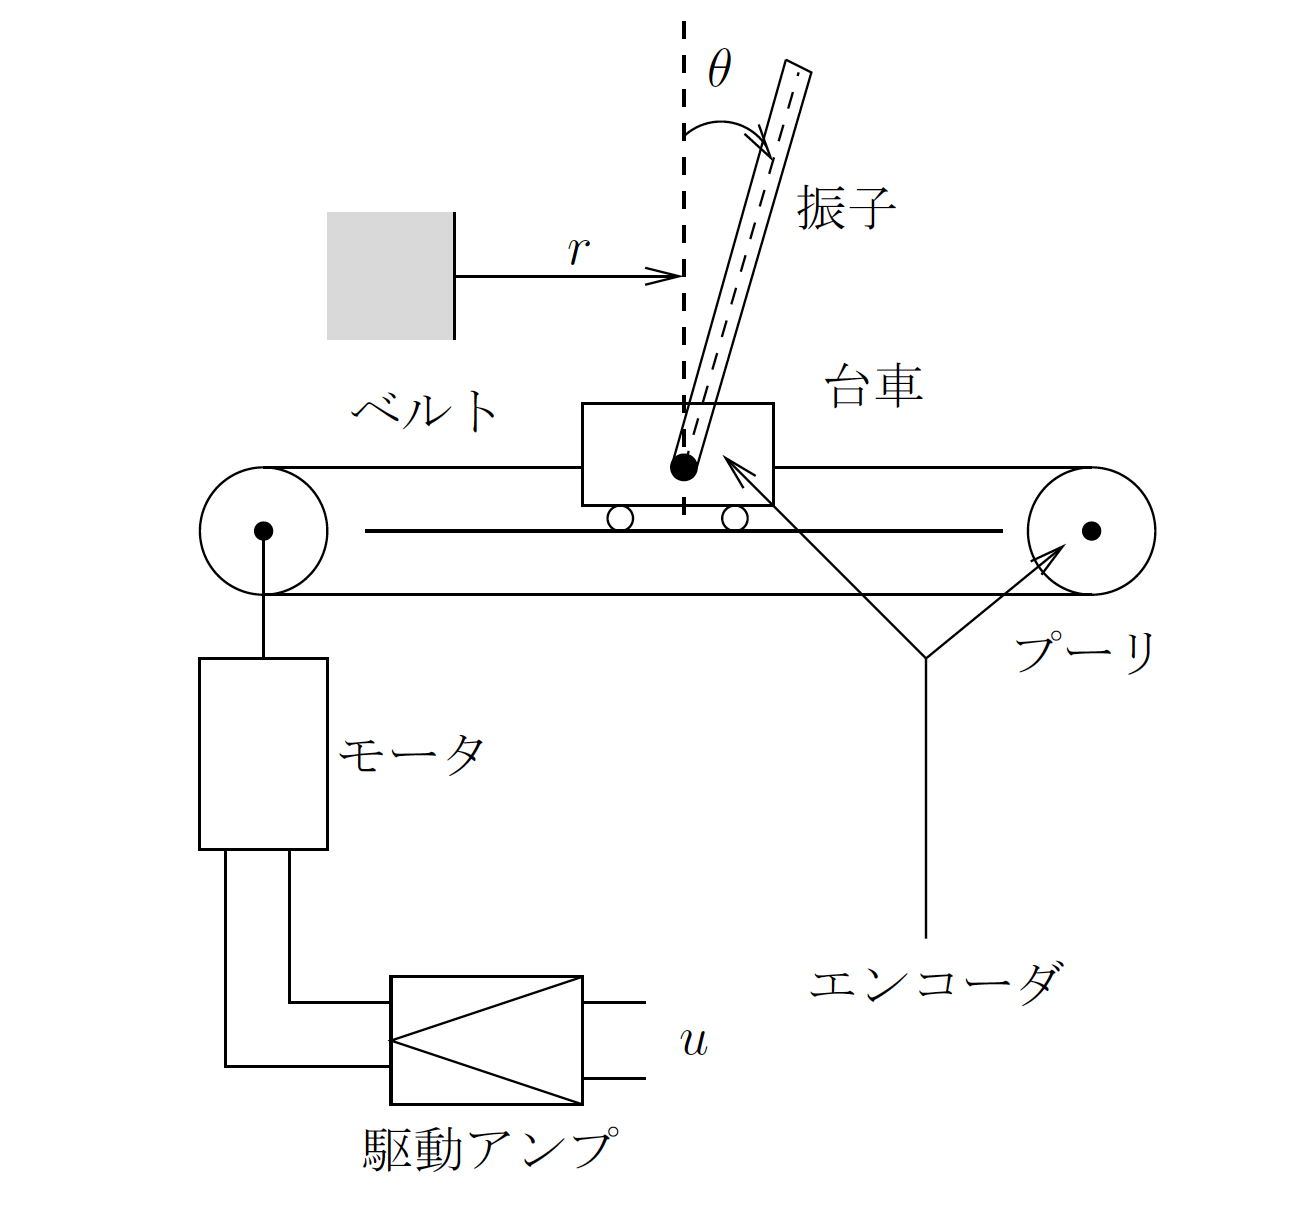
\includegraphics[width = 0.6 \linewidth]{model.png}
		\caption{倒立振子系}
		\label{fig:倒立振子系}
	\end{center}
\end{figure}

\chapter{モデリング}
\section{数式モデル}
制御目的を達成する制御システムを設計するためにまず、倒立振子系について、状態方程式と観測方程式から成る数式モデルを導出する。
\subsection{状態方程式}
% 2.1図の挿入
\begin{figure}[htbp]
	\begin{center}
		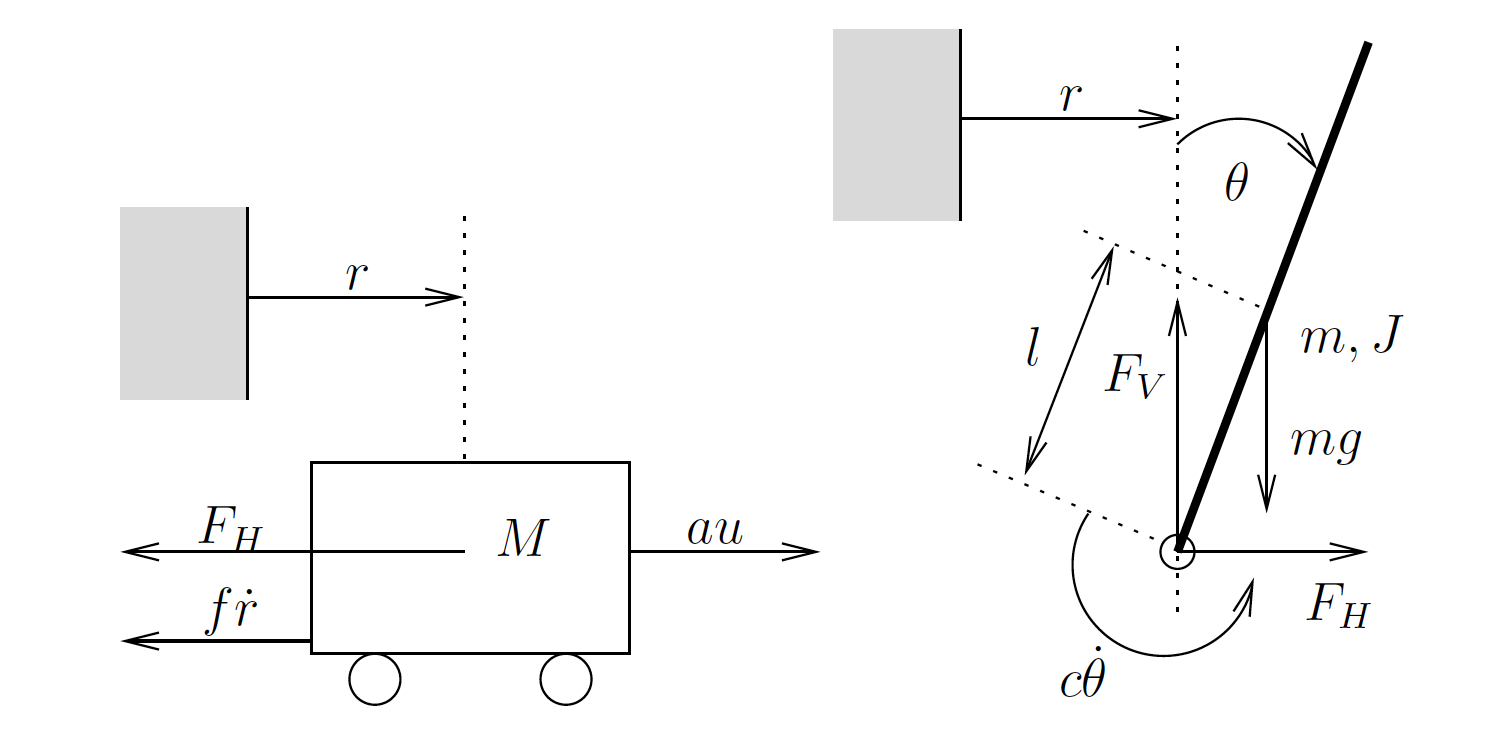
\includegraphics[width = 0.6 \linewidth]{modeling.png}
		\caption{数学モデル導出のための参考図}
		\label{fig:数式モデル導出のための参考図}
	\end{center}
\end{figure}

図\ref{fig:数式モデル導出のための参考図}を参照して、台車と振子に関する運動方程式がつぎのように得られる。

\begin{eqnarray}
&&M \ddot{r} = au - F_H - f \dot{r}
\label{eq:2.1}\\
&&J \ddot{\theta} = lF_V\sin{\theta} - lF_H\cos{\theta} - c\dot{\theta}
\label{eq:2.2}\\
&&m \frac{d^2}{dx^2} (r + l\sin(\theta))  =  F_H
\label{eq:2.3}\\
&&m \frac{d^2}{dx^2} (l\cos(\theta))  =  F_V - mg
\label{eq:2.4}
\end{eqnarray}
ここで、$M,f$は台車の質量と摩擦係数、$m,l,J,c$は振子の質量、回転軸・重心間距離、重心まわり慣性モーメント、回転軸摩擦係数、$F_H,F_V$は振子が台車から受ける水平抗力と垂直抗力である。また、$u$は駆動アンプへの入力電圧、$a$は駆動アンプへの入力電圧から台車への駆動力までのゲインである。

いま、4つの状態変数から成るベクトル、すなわち状態$x$を
\begin{eqnarray}
	x=\left[
	\begin{array}{c}
		r\\
		\theta\\
		\dot{r}\\
		\dot{\theta}
	\end{array}
	\right]
\end{eqnarray}
のように定義すると、、(\ref{eq:2.1})-(\ref{eq:2.4})式から、倒立振子系の非線形状態方程式を求める。
(\ref{eq:2.1})に(\ref{eq:2.2})を代入すると

\begin{eqnarray}
	M\ddot{r} = au - m\ddot{r}+ml\sin{\theta}-f\dot{r}
\end{eqnarray}
\begin{eqnarray}
\ddot{r} = \frac{au + ml\sin{\theta}-f\dot{r}}{M+m}
\label{eq:rddot}
\end{eqnarray}
また、(\ref{eq:2.2})に(\ref{eq:2.3}),(\ref{eq:2.4})を代入すると
\begin{eqnarray}
	J\ddot{\theta} = l\left(m\frac{d^2}{dt^2}(l\cos{\theta}+mg) \right)\sin{\theta}
	- l \left( m\frac{d^2}{dt^2}(r+l\sin{\theta}) \right)\cos{\theta}
\end{eqnarray}
\begin{eqnarray}
ml\cos{\theta}\ddot{r}+(J+ml^2)\ddot(\theta)=mgl\sin{\theta}-c\dot{\theta}
\label{eq:rddot,thddot}
\end{eqnarray}
(\ref{eq:rddot}),(\ref{eq:rddot,thddot})を行列式で表すと
\begin{eqnarray}
	\left[
	\begin{array}{cc}
		M+m & ml\cos{\theta}\\
		ml\cos{\theta} & J+ml^2
	\end{array}
	\right]
	\left[
	\begin{array}{c}
		\ddot{r} \\
		\ddot{\theta}
	\end{array}
	\right] =
	\left[
	\begin{array}{c}
		- f \dot{r} + ml\sin{\theta}・\dot{\theta}^2 + au\\
		mgl\sin{\theta} - c\dot{\theta}
	\end{array}
	\right]\\
	\left[
	\begin{array}{c}
		\ddot{r} \\
		\ddot{\theta}
	\end{array}
	\right] =
	\left[
	\begin{array}{cc}
		M+m & ml\cos{\theta}\\
		ml\cos{\theta} & J+ml^2
	\end{array}
	\right]^{-1}
	\left[
	\begin{array}{c}
		- f \dot{r} + ml\sin{\theta}・\dot{\theta}^2 + au\\
		mgl\sin{\theta} - c\dot{\theta}
	\end{array}
	\right]
\end{eqnarray}
よって、
%(5)
\begin{eqnarray}
\dot{x}=f(x,u)=\left[
\begin{array}{c}

\dot{r}\\
\dot{\theta}\\
K^{-1}\left[
\begin{array}{c}
- f \dot{r} + ml\sin{\theta}・\dot{\theta}^2 + au\\
mgl\sin{\theta} - c\dot{\theta}
\end{array}
\right]

\end{array}
\right],\,
K = \left[
\begin{array}{cc}
M+m & ml\cos{\theta}\\
ml\cos{\theta} & J+ml^2
\end{array}
\right]
\end{eqnarray}
のように得られる。

ところで、倒立振子系については、その制御目的から、不安定平衡点$x=0$の近傍での挙動を表す方程式を知れば充分である。そこで、この基準状態まわりで一次近似された状態方程式を求めることを考える

倒立振子系に対する状態方程式は、つぎのように得られる。
%(6)
\begin{eqnarray}
\dot{x} = Ax + Bu
\label{eq:xdot}
\end{eqnarray}
ここで

\begin{eqnarray}
	A = \left[
	\begin{array}{cc}
		0_{2×2} & I_2\\
		A_{21} & A_{22}
	\end{array}
	\right],\,
	B = \left[
	\begin{array}{c}
		0_{2×2}\\
		B_2
	\end{array}
	\right]\\
\end{eqnarray}
ただし

\begin{eqnarray}
	A_{21} = K^{-1}\left[
	\begin{array}{cc}
		0 &  0 \\
		0 & mgl
	\end{array}
	\right],\,
	A_{22} = K^{-1}\left[
	\begin{array}{cc}
		-f &  0 \\
		0 & -c
	\end{array}
	\right],\,
	B_{2} = K^{-1}\left[
	\begin{array}{c}
		a\\
		0
	\end{array}
	\right]
\end{eqnarray}

\begin{eqnarray}
	K = \left[
	\begin{array}{cc}
		M+m & ml \\
		ml & J+ml^2
	\end{array}
	\right]
\end{eqnarray}

\subsection{観測方程式}
2つの観測出力は
\begin{eqnarray}
	y_1 = c_1r\\
	y_2 = c_2\theta
\end{eqnarray}
のように表される。ここで$c_1$は変位・電圧変換係数、$c_2$は角度・電圧変換係数である。これから成るベクトルすなわち出力$y$を

\begin{eqnarray}
	y = \left[
	\begin{array}{c}
		y_1\\
		y_2
	\end{array}
	\right]
\end{eqnarray}
のように定義すると、倒立振子系に対する観測方程式として

\begin{eqnarray}
	y = Cx
\end{eqnarray}
ただし

\begin{eqnarray}
C = \left[
\begin{array}{cc}
N & 0_{2×2}
\end{array}
\right] = \left[
\begin{array}{cccc}
c_1 &  0  & 0 & 0\\
0  & c_2 & 0 & 0
\end{array}
\right],\,
N = \left[
\begin{array}{cc}
c_1 &  0 \\
0  & c_2
\end{array}
\right]
\label{eq:C,N}
\end{eqnarray}
を得る。

\section{物理パラメータの決定}
\subsection{$m$と$l$の測定}
振子を装置から取り外し、バネ秤で$m$を測定しなさい。つぎに、振子を鋼尺のエッジ上で
バランスさせて、重心の位置を定め、$l$を測定する。

\subsection{$c_1$と$c_2$の測定}
$c_1$と$c_2$は、
\begin{eqnarray}
	c_1 = 1.0\\
	c_2 = 1.0
\end{eqnarray}
のようにソフトウェア内で設定済みである。

\subsection{$a$の測定}
モータに一定電圧を加え、バネばかりで台車を引き、台車が正の方向に動き出すときの力($au+摩擦力$)を$f_{max}$、負の方向に動き出すときの力($au+摩擦力$)を$f_{min}$とする。図\ref{fig:パラメータaの決定}にしめすように$u$と$f_{max},f_{min}$の関係をいくつかの電圧について調べ、最小2乗法によって1次関数を求め、この傾きを$a$とする。


% 2.2図の挿入
\begin{figure}[htbp]
	\begin{center}
		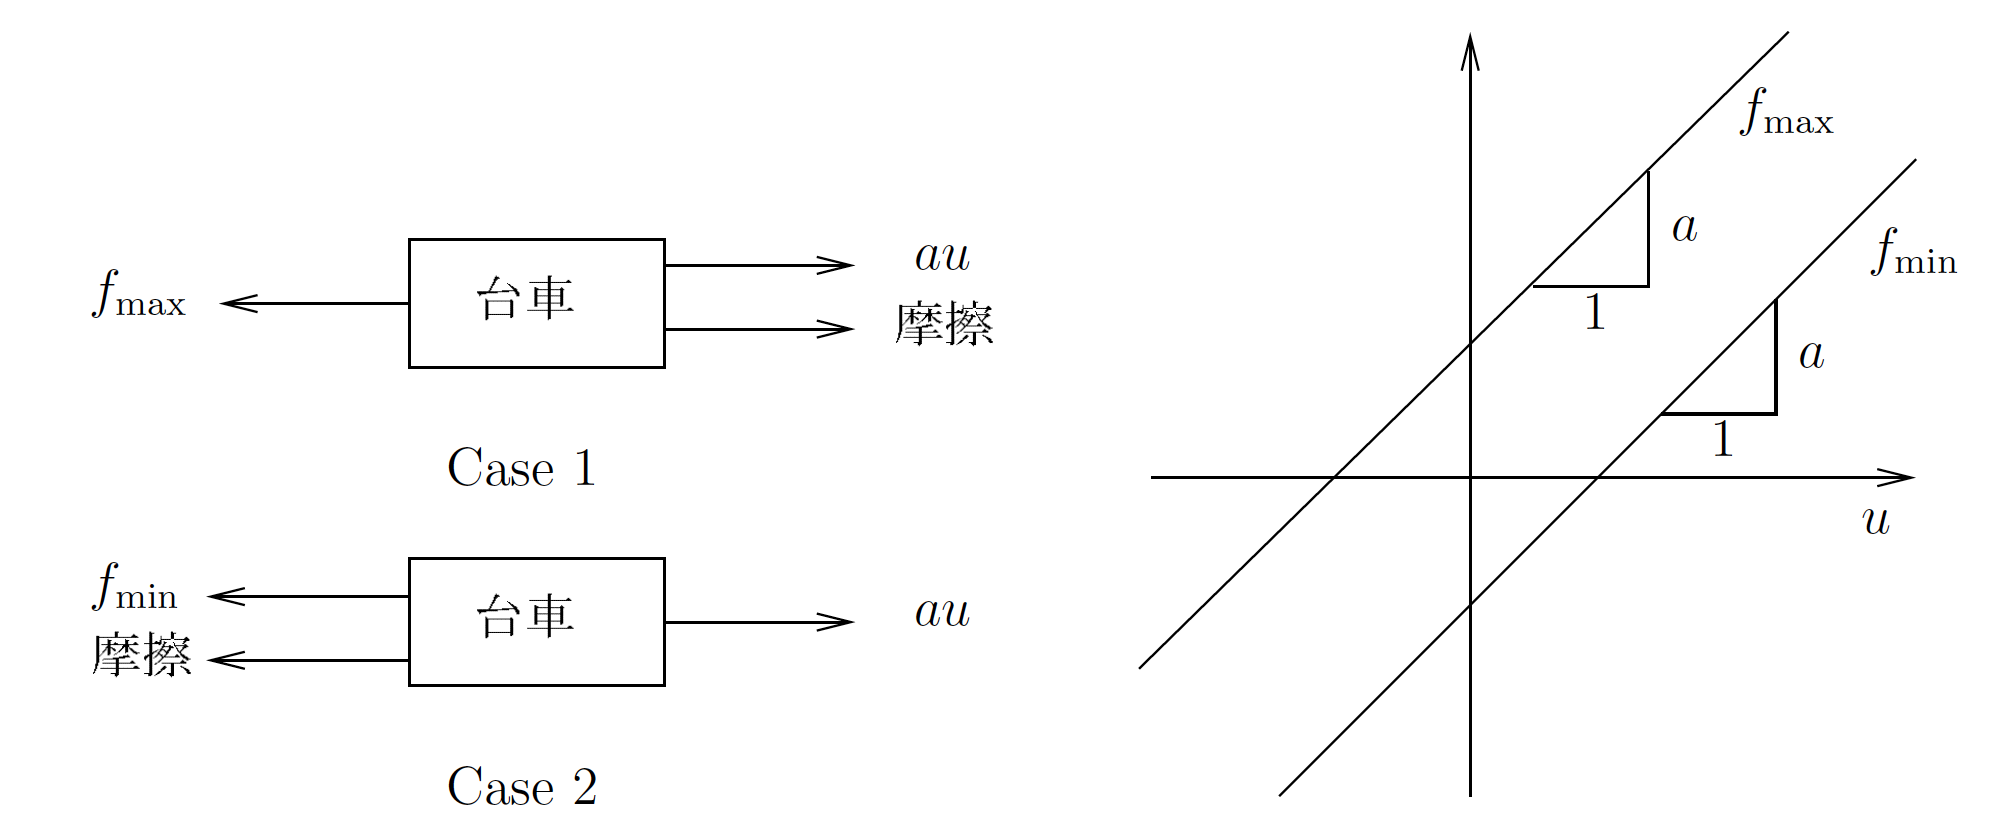
\includegraphics[width = 0.8 \linewidth]{definition_a.png}
		\caption{パラメータaの決定}
		\label{fig:パラメータaの決定}
	\end{center}
\end{figure}

\subsection{ステップ応答による$M$と$f$の測定}

% 2.3図の挿入
\begin{figure}[htbp]
	\begin{center}
		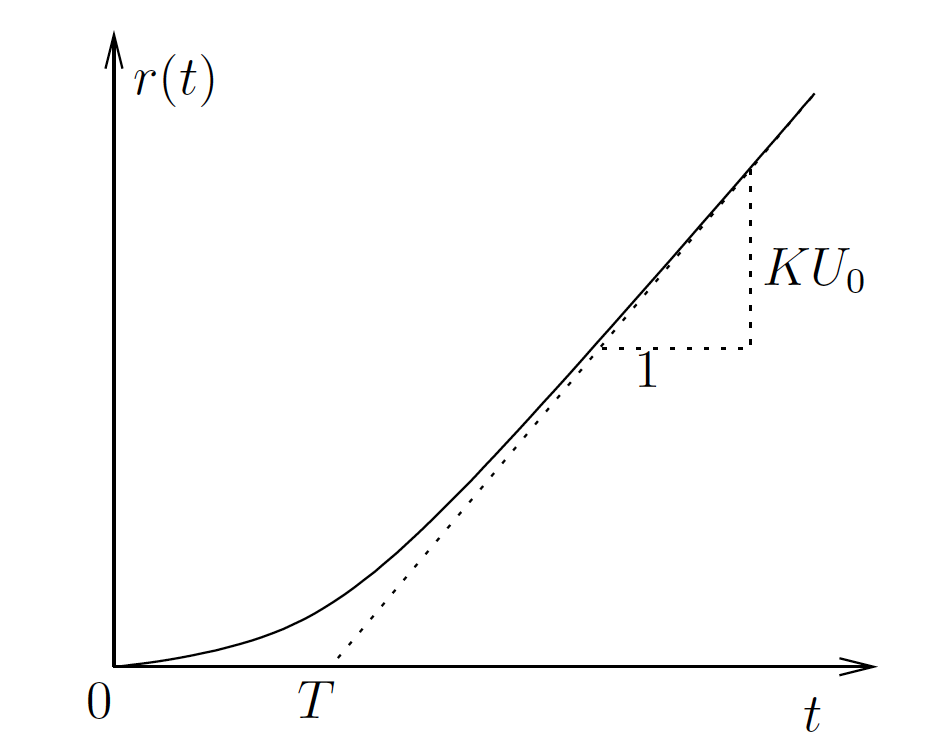
\includegraphics[width = 0.6 \linewidth]{cart_step.png}
		\caption{台車のステップ応答}
		\label{fig:台車のステップ応答}
	\end{center}
\end{figure}

振子を台車から取り外して、台車のステップ応答を測定する。そのときの運動方程式は
\begin{eqnarray}
	M\ddot{r} = au - fr
\end{eqnarray}
であり、$u$から$r$までの伝達関数$G$を求めると
\begin{eqnarray}
	G(s) = \frac{K}{s(Ts+1)}
\end{eqnarray}
となる。だたし、
\begin{eqnarray}
K = \frac{a}{f},T = \frac{M}{f}
\label{eq:K,T}
\end{eqnarray}
である。初期状態をゼロとするとき、このシステムのステップ応答は
\begin{eqnarray}
r(t) = KU_o(T\exp{\frac{-t}{T}}+t-T)
\label{eq:r(t)}
\end{eqnarray}
である。(図\ref{fig:台車のステップ応答}参照)。$U_0$はステップの高さである。(\ref{eq:r(t)})式において$t→∞$とすれば
\begin{eqnarray}
r(t) = KU_o(t-T)
\end{eqnarray}
となり、これから$T$と$K$をもとめ(図\ref{fig:台車のステップ応答}参照)、(\ref{eq:K,T})式より$M$と$f$を決定することができる。

\subsection{フィードバック制御による$M$と$f$の測定}
台車は外見は小さいが、台車を手で動かしてみると、かなり重たい。これはモータ(ギア付)の軸のトルクがあるためである。そこで、$M$と$f$は、アンプ・モータ・プーリ・ベルト・台車系の等価質量と等価摩擦係数として計測する。

\begin{figure}[htbp]
	\begin{center}
		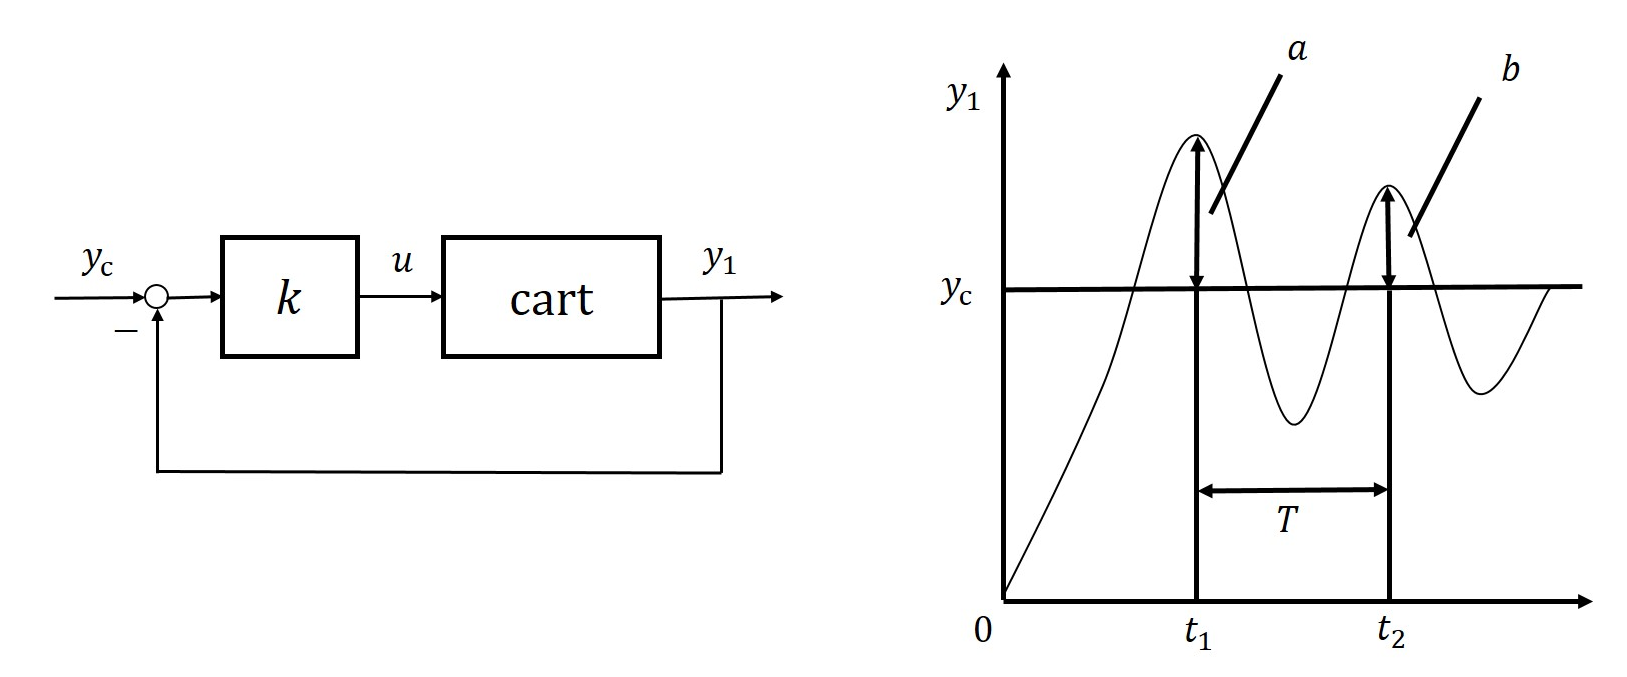
\includegraphics[width = 1.0 \linewidth]{feedback.eps}
		\caption{台車のフィードバック応答}
		\label{fig:台車のフィードバック応答}
	\end{center}
\end{figure}

台車の数式モデルは
\begin{eqnarray}
	M\ddot{r} & = & au - fr \\
	y_1 & = & c_1r
\end{eqnarray}
である。これに図\ref{fig:台車のフィードバック応答}に示すようにフィードバック
\begin{eqnarray}
	u = k(y_c - y_1)
\end{eqnarray}
を施すと$(y_cは定数,k>0)$、閉ループシステムの応答は
\begin{eqnarray}
	M\ddot{y}_1 + f\dot{y}_1 + c_1aky_1 = c_1aky_c
\end{eqnarray}
に従う。一方、偏差$z$を

\begin{eqnarray}
	z = y_1 - y_c
\end{eqnarray}
により定義すると、これは
\begin{eqnarray}
	\ddot{z} + 2\zeta\omega_n\dot{z} + \omega_n^2z = 0
\end{eqnarray}
ただし
\begin{eqnarray}
\zeta = \frac{f}{2\sqrt{c_1akM}} , \omega_n = \sqrt{\frac{c_1ak}{M}}
\label{eq:ZETA,OMEGA}
\end{eqnarray}
に従う。この解は
\begin{eqnarray}
	0 < \zeta < 1
\end{eqnarray}
このとき、減衰振動となり
\begin{eqnarray}
	z(t) = \frac{z_0}{\sqrt{1-\zeta^2}}\exp(-\omega_n\zeta
	t)\,\sin(\omega_n\sqrt{1-\zeta^2}\,t+\phi)
\end{eqnarray}
ただし
\begin{eqnarray}
	\phi = \tan^{-1}{\frac{\sqrt{1-\zeta^2}}{\zeta}}
\end{eqnarray}
で与えられる。ここで、$z_0 = z(0) = -y_c$である。いま、$T$とし、
時刻$t_1$と$t_2 = t_1 + T$において波形$z$の山が隣合うものとする。
このときの振幅の減衰比は
\begin{eqnarray}
	\frac{|z_2(t_2)|}{|z_2(t_1)|} = \exp(-\lambda)
\end{eqnarray}
ただし
\begin{eqnarray}
\lambda = \frac{2\pi\zeta}{\sqrt{1-\zeta^2}}
\label{eq:LAMBDA}
\end{eqnarray}
となる。この$\lambda$は対数減衰比と呼ばれる。また
\begin{eqnarray}
T = \frac{2\pi}{\omega_n\sqrt{1-\zeta^2}}
\label{eq:T}
\end{eqnarray}
が成り立つ。したがって、(\ref{eq:ZETA,OMEGA})と(\ref{eq:LAMBDA}),(\ref{eq:T})から、$M$と$f$は
\begin{eqnarray}
M = \frac{c_1akT^2}{4\pi^2 + \lambda^2},f = \frac{2\lambda M}{T}
\label{M,f}
\end{eqnarray}
のように与えられる。

\subsection{$J$と$c$の測定}
振子を自由振動させることにより、$J$と$c$を測定できる。その数式モデルは
\begin{eqnarray}
(J+ml^2)\ddot{\theta} & = & -mgl\sin{\theta} - c\dot{\theta}
\label{eq:J,c1}\\
y_2 & = & c_2\theta
\label{eq:J,c2}
\end{eqnarray}
で与えられる。$\theta$を微小範囲で考えると、(\ref{eq:J,c1})-(\ref{eq:J,c2})式は
\begin{eqnarray}
	\ddot{y}_2 + 2\zeta\omega_n\dot{y_2} + \omega_n^2y_2 = 0
\end{eqnarray}
ただし
\begin{eqnarray}
	\zeta = \frac{c}{2\sqrt{mgl(J + ml^2)}},\,
	\omega_n = \sqrt{\frac{mgl}{J + ml^2}}
\end{eqnarray}
のように書くことができる。この解で表される減衰振動の対数減衰率を$\lambda$、周期を$T$とすると、
関係式(\ref{eq:LAMBDA}),(\ref{eq:T})が成り立つことから、$J,c$は
\begin{eqnarray}
J = \frac{mglT_2^2}{4\pi^2 + \lambda^2} - ml^2 ,\, c = \frac{2\lambda(J +
	ml^2)}{T}
\end{eqnarray}
のように与えられる。

\clearpage

\begin{figure}[htbp]
	\begin{center}
		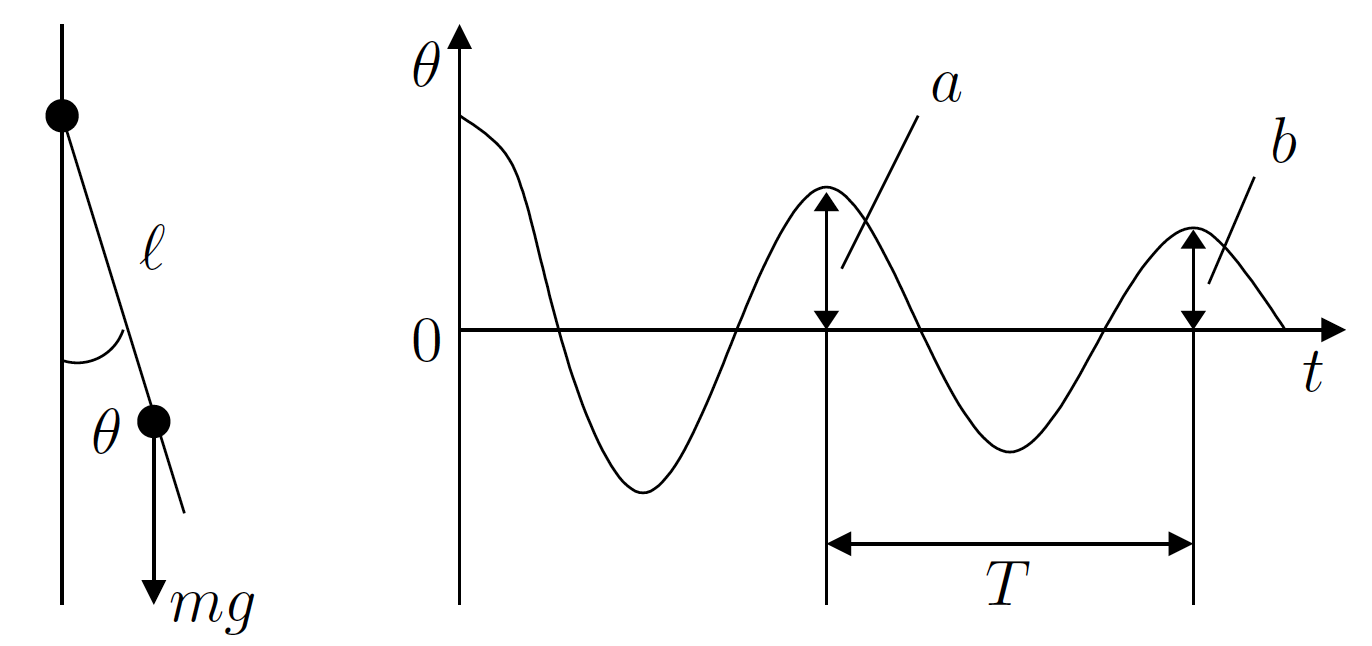
\includegraphics[width = 0.7 \linewidth]{measure_jc.png}
		\caption{振子の自由振動}
		\label{fig:振子の自由振動}
	\end{center}
\end{figure}


\section{パラメータの検証}

\chapter{制御系設計}
\begin{figure}

\end{figure}
\section{特性解析}
\section{制御システムの構成}
\section{$F$の設計}
\section{$\hat{A}$,$\hat{B}$,$\hat{J}$,$\hat{C}$,$\hat{D}$の設計}
\section{離散化}
\section{振り上げ制御}	

\chapter{シミュレーション}
\section{安定化制御}
\section{振り上げ制御}

\chapter{実験}
\section{実験装置}
\section{安定化制御}
\section{振り上げ制御}
\section{考察}

\chapter{おわりに}

\end{document}